\documentclass{article}
\setlength{\parskip}{0pt} % esp. entre parrafos
\setlength{\parindent}{3pt} % esp. al inicio de un parrafo
\usepackage{amsmath} % mates
\usepackage{listings}
\usepackage[sort&compress,numbers]{natbib} % referencias
\usepackage{url} % que las URLs se vean lindos
\usepackage[top=15mm,left=20mm,right=20mm,bottom=25mm]{geometry} % \textbf{\textbf{}}margenes
\usepackage{hyperref} % ligas de URLs
\usepackage{graphicx} % poner figuras
\usepackage{subfigure}
\usepackage[spanish]{babel} % otros idiomas
\hypersetup{
    colorlinks=true,
    linkcolor=blue,
    filecolor=blue,      
    urlcolor=blue,
    citecolor=black,
}

\title{TAREA \# 11 \\ Frentes de Pareto} %titulo
\author{Natalia Berenice P\'{e}rez L\'{o}pez} % author
\date{\today}

\begin{document} % inicia contenido

\maketitle % cabecera

\section{Objetivo}
El objetivo de esta práctica es graficar el porcentaje de soluciones de Pareto (ojo, no es lo mismo que se grafica en el código ejemplo) como función del número de funciones objetivo con diagramas de violín combinados con diagramas de caja-bigote, verificando que diferencias observadas, cuando las haya, sean estadísticamente significativas. Razona en escrito a qué se debe el comportamiento observado.

\section{Desarrollo} % seccion y etiqueta
Para generar el código de esta práctica se realizaron algunas ideas y pruebas iniciales, las cuales se encuentran en \href{https://github.com/nataliaperez0/Simulation/tree/main/Tarea11}{mi repositorio}  en GitHub. Se inició tomando como base el código para obtener el frente de Pareto \citep{1} y el código para realizar gráficas de violín \citep{2}, ambos revisados en clase. Las modificaciones que se le realizaron al código fueron: establecer un vector con las cantidades de funciones objetivo, agregar un ciclo \texttt{for} para variar dichas cantidades y otro para hacer $20$ réplicas de cada cantidad de objetivos, también se agregó el código para obtener el porcentaje de soluciones Pareto y un \texttt{data.frame} para almacenar el valor de $k$, el número de réplica y el porcentaje correspondiente.
\bigskip

A continuación se muestra el fragmeto modificado en el código: 

\definecolor{verde}{rgb}{0,0.56,0.22}
\definecolor{codegray}{rgb}{0.5,0.5,0.5}
\definecolor{codegreen}{rgb}{0,0.56,0.22}
\definecolor{backcolour}{rgb}{0.95,0.95,0.92}
\definecolor{azul}{rgb}{0,0,1}

\lstdefinestyle{mystyle}{
    backgroundcolor=\color{backcolour},   
    commentstyle=\color{verde},
    keywordstyle=\color{azul},
    numberstyle=\tiny\color{codegray},
    stringstyle=\color{codegreen},
    basicstyle=\ttfamily\footnotesize,
    breakatwhitespace=false,         
    breaklines=true,                 
    captionpos=b,                    
    keepspaces=true,                 
    numbers=left,                    
    numbersep=5pt,                  
    showspaces=false,                
    showstringspaces=false,
    showtabs=false,                  
    tabsize=2
}

\lstset{style=mystyle}
\begin{lstlisting}[language=R, caption= Fragmento del código modificado.]
df = data.frame()
vc <- 4
md <- 3
tc <- 5
funciones <- c(2, 3, 4, 5) # cuantas funciones objetivo
obj <- list()
k = 0

for (j in funciones){
  k = j
  for (replica in 1:20){
    for (i in 1:k) {
      obj[[i]] <- poli(md, vc, tc)
    }
    minim <- (runif(k) > 0.5)
    sign <- (1 + -2 * minim) # neg -> min, pos -> max
    n <- 200 # cuantas soluciones aleatorias
    sol <- matrix(runif(vc * n), nrow=n, ncol=vc)
    val <- matrix(rep(NA, k * n), nrow=n, ncol=k)
    for (i in 1:n) { # evaluamos las soluciones
      for (j in 1:k) { # para todos los objetivos
        val[i, j] <- eval(obj[[j]], sol[i,])
      }
    }
    mejor1 <- which.max(sign[1] * val[,1])
    mejor2 <- which.max(sign[2] * val[,2])
    cual <- c("max", "min")
    no.dom <- logical() # TRUE/FALSE segun si nadie lo domina
    dominadores <- integer()
    for (i in 1:n) { # para cada asignacion
      d <- logical() # quienes le dominan (si / no)
      for (j in 1:n) { # para todos los demas
        d <- c(d, domin.by(sign * val[i,], sign * val[j,]))
      }
      cuantos <- sum(d)
      dominadores <- c(dominadores, cuantos)
      no.dom <- c(no.dom, sum(d) == 0) # nadie le domina (puros FALSE)
    }
    frente <- subset(val, no.dom) # solamente las no dominadas
    porcentaje = (length(frente[,1])/n)*100
    resultado = c(k, replica, porcentaje)
    df = rbind(df, resultado)
    names(df) = c("k", "Replica", "Porcentaje")
  }
}
\end{lstlisting}

Utilizando el \texttt{data.frame} obtenido con el código anterior se realizó el diagrama caja-bigote combinado con diagramas de violín para analizar como varía el porcentaje de soluciones Pareto al incrementar el número de funciones objetivo (Ver figura \ref{f1}).  

\begin{figure} [h!]% figura
    \centering
    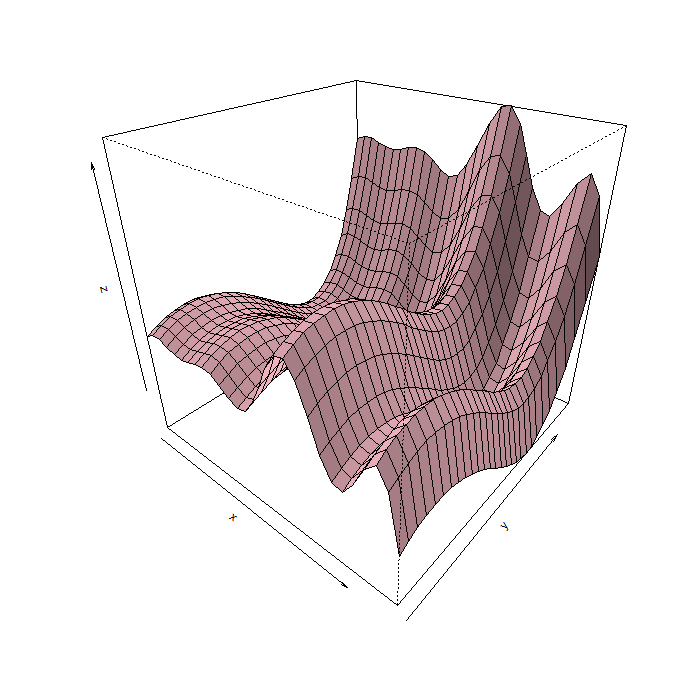
\includegraphics[width=150mm]{Figura1.png} % archivo
    \caption{Porcentaje de soluciones de Pareto que se obtienen con cada cantidad de funciones objetivo $k$.}
    \label{f1}
\end{figure}

\newpage
En la figura \ref{f1} se puede observar que con mayores cantidades de funciones objetivo se tienen más soluciones en el frente de Pareto. Para analizar si existe una relación entre la variación del número de funciones objetivo $k$ y el porcentaje de soluciones en el frente de Pareto se realizó una prueba estadística. Se eligió realizar la prueba estadística \texttt{Kruskal Wallis} debido a que los datos no presentan normalidad.
\bigskip

En el cuadro \ref{Cuadro1} se  resumen los resultados de la revisión de los supuestos para poder aplicar la prueba estadística. El supuesto outliers se refiere a la cantidad de valores atípicos que existen en los grupos, la normalidad por grupos se obtuvo con la prueba de \texttt{Shapiro Wilk} y la homogeneidad de varianza se obtuvo con la prueba de \texttt{Levene}.

\begin{table}[ht]
\centering
\caption{Resultados del los supuestos para aplicar la prueba estadística.}
\smallskip

\begin{tabular}{ |p{2.1cm}|p{2.1cm}|}
 \hline
 Outliers & $2$ \\
 \hline
 Normalidad por grupo & $2$: $p$ = $0.0003$ $3$: $p$ = $0.0104$ $4$: $p$ = $0.1990$ $5$: $p$ = $0.0383$ \\
 \hline
 Homogeneidad de varianza & $p$ = $1.9\times 10^{-5}$ \\
 \hline
\end{tabular}
\label{Cuadro1}
\end{table}

En los resultados se observa que para la normalidad en tres de los cuatro grupos $p$ es menor a $0.05$, por lo tanto no se tiene normalidad.
\bigskip

Al realizar la prueba \texttt{Kruskal Wallis} se obtienen los resultados mostrados en el cuadro \ref{Cuadro2}.

\begin{table}[h!]
\centering
\caption{Resultados al aplicar la prueba estadística \texttt{Kruskal Wallis}.}
\smallskip

\begin{tabular}{ |p{2.1cm}|p{2.1cm}|}
 \hline
 Chi cuadrada & Valor de $p$ \\
 \hline
 $45.369$ & $7.72\times 10^{-10}$ \\
 \hline
\end{tabular}
\label{Cuadro2}
\end{table}

Hipótesis nula : Las medias son iguales en todos los grupos.
\smallskip

Hipótesis alternativa: Debido a que $p < 0.05$ se rechaza la hipótesis nula, es decir que si existen diferencias significativas entre las medias de los grupos. 
\bigskip

Se entiende entonces que el aumentar la cantidad de funciones objetivo si tiene un efecto significativo en la cantidad de soluciones en el frente de Pareto.
\bigskip

También podemos realizar la prueba de suma de rangos de \texttt{Wilcoxon} por pares para observar los resultados de $p$ y determinar si existen diferencias al comparar entre ellos los valores de $k$ (Ver cuadro \ref{Cuadro3}).

\begin{table}[ht]
\centering
\caption{Resultados al aplicar la prueba \texttt{Wilcoxon}.}
\smallskip

\begin{tabular}{|p{1.7cm}|p{1.7cm}|p{1.7cm}|p{1.7cm}|}
 \hline
Valor de $p$ & $2$ & $3$ & $4$ \\
 \hline
 $3$ & $1.5\times 10^{-4}$ & - & - \\
 \hline
 $4$ & $3.7\times 10^{-5}$ & $0.03089$ & -\\
 \hline
 $5$ & $6.3\times 10^{-7}$ & $9.7\times 10^{-5}$ & $0.04018$ \\
 \hline
\end{tabular}
\label{Cuadro3}
\end{table}

En los resultados de la prueba podemos observar que todos los valores de $p$ son menores a $0.05$ lo cual indica que entre todos los grupos sí existen diferencias significativas en sus medias.
\bigskip

A continuación se muestra el código utilizado para realizar la figura \ref{f1} y la prueba estadística \texttt{Kruskal Wallis}:

\lstset{style=mystyle}
\begin{lstlisting}[language=R, caption= Código para graficar y realizar las pruebas estadísticas \texttt{Kruskal Wallis} y \texttt{Wilcoxon}.]
library(ggplot2)
df$k = as.factor(df$k)
png("Figura1.png", width=15, height=15, units="cm", res=1200)
gr <- ggplot(df, aes(x=k, y=Porcentaje)) + geom_violin(fill="pink", color="purple")
gr + geom_boxplot(width=0.2, fill="cyan", color="black", lwd=0.5) +
  labs(x = "Cantidad de funciones objetivo", y = "% de soluciones Pareto")
graphics.off()

library(tidyverse)
library(ggpubr)
library(car)
library(rstatix)
library(rapportools)
library(readr)
library(gridExtra)

#PRUEBA ESTADISTICA...
#Estadisticas descriptivas
df %>%
  group_by(k) %>%
  get_summary_stats(Porcentaje, type = "mean_sd")

#SUPUESTOS PARA ANOVA
#1:Outliers
df %>%
  group_by(k) %>%
  identify_outliers(Porcentaje)

#2:Normalidad por Shapiro
df %>%
  group_by(k) %>%
  shapiro_test(Porcentaje)

#3:Homogeneidad de varianza con prueba Levene
df %>%
  levene_test(Porcentaje~k)

#PRUEBA ESTADISTICA KRUSKAL WALLIS
kruskal.test(Porcentaje ~ k, data = df)

#PRUEBA WILCOXON
pairwise.wilcox.test(df$Porcentaje, df$k)
\end{lstlisting}

\newpage

\section{Conclusi\'{o}n}
Con base en el diagrama caja-bigote combinado con los diagramas de violín y con los resultados de la prueba estadística puedo concluir que el porcentaje de soluciones de Pareto aumenta cuando se tienen más funciones objetivo, podemos observar que con solo dos funciones objetivo el frente de Pareto se compone de menos del $25\%$ de las soluciones totales, sin embargo con cinco funciones objetivo el frente de Pareto puede considerarse casi la totalidad de las soluciones, llegando a tener más del $75\%$ de las soluciones, esto se debe principalmente a que con más funciones objetivo existen más combinaciones que pueden considerarse en el frente de Pareto aunque solo cuenten con algunos de los objetivos óptimizados. Lo a
\smallskip

En general ésta práctica me pareció sencilla de comprender y con muchas aplicaciones en la realidad.
\newpage

\bibliography{referencias}
\bibliographystyle{plainnat}

\end{document}